\documentclass[12pt]{article}

\usepackage{graphicx}
\usepackage[doublespacing]{setspace}
\usepackage{textcomp}
\usepackage{amsmath}
\usepackage{amssymb}
\usepackage{fancyhdr}
\usepackage{lastpage}
\usepackage{float}
\usepackage{array}
\usepackage{indentfirst}
\usepackage{titletoc}
\titlecontents{chapter}[0pt]{\addvspace{2pt}\filright}
              {\contentspush{\thecontentslabel\ }}
              {}{\titlerule*[8pt]{.}\contentspage}
\setlength{\parindent}{2em}
\pagestyle{fancy}
\lhead{Team \# 61416}
\rhead{Page \thepage{} of \pageref{LastPage}}
\cfoot{}

\begin{document}
\begin{center}
{\Large Optimizing the Passenger Throughput --Based on Network-Flows }
\end{center}


\begin{abstract}
\setlength{\parindent}{0pt} \setlength{\parskip}{1.5ex plus 0.5ex
minus 0.2ex}
For the airport management, it is a real-life common phenomenon to save passengers' time as far as possible. An appropriately example is that sometimes passengers who arrive airport later may not board the flight because of the low efficiency of checkpoints. Therefore we need a model to test and discover the bottlenecks of airport checkpoint efficiency and propose the existing system a number of feasible modifications to improve efficiency. Our model for this problem is the Network-Flows. Applying the Edmonds-Karp algorithm, we obtain the maximum efficiency of the airport security system proportional to the efficiency through making the network traffic and airport security system. And then observe the modified maximum traffic of the network changes after modifying some of the parameters of the network. If some big changes have occurred, it is indicated that this part is more likely to affect the airport security efficiency bottlenecks. After that, we can try to make some modifications to the network without changing its basic parameters so that the maximum traffic is larger than before. So we can identify potential, feasible and excellent programs using the mapping relation between the network and airport security system. Finally, we consider comprehensive factors to evaluate the modified program's merits and drawbacks.
\end{abstract}

\tableofcontents

\clearpage
\setlength{\parindent}{2em}
\section{Introduction}


In order to solve the problem of security's low efficiency, the airport introduces the ``Pre-Check". With the rapid increase of the number of Pre-Check passengers many people may think that, can we directly increase Pre-Check channels to improve efficiency? However, practical questions are not as simple as imagined. What's more, in the additional data set, is the given data really enough for us to solve the problem? What will happen to the efficiency of the airport security system if the machine to screen or identify passenger's identity break out? When passengers line up in the case that there are not merely one choice, is there a different efficiency of airport security system if passenger choose a different channel? Against so many factors, how we should comprehensively adapt them to accommodate passenger growth and other cases?
\section{Description and Application}

\setlength{\parindent}{2em}
We use the Network-Flows model to abstract this practical problem. Essentially Network-Flows model is a directed graph. There are edges between points and each edge has a parameter V called capacity, `which expresses the largest flow to the edges' direction. Generally, the Network-Flows model has a source point which is the beginning of the traffic, can be understood as a water source and a meeting point where traffic is collected here. So the final flow to the sink is the largest Network-Flow. Seeking the maximum flow of Network-Flow is the most classic application of the Network-Flows.

As mentioned above, we can apply Network-Flows to the practical questions as followed:
The airport can be seen as the source point, and the security exit is the meeting point. The question's require of more security capacity in a shorter period of time, in another view, is the larger number of more people passing the checkpoints per unit time. Apparently, the larger the capacity is, the more superior corresponding program is. Thus, calculate the passing passengers number each step per unit time and we can abstract them into the value of traffic capacity. So that each step can be abstracted into an edge of the net and edge capacity is the passing passenger quantity of the step, the points in the net become the place before the beginning of the corresponding steps.
In summary, we can build the final net. So the result of Edmonds-Karp is the current program's largest number that passing the checkpoints.

\section{Assumptions}

\setlength{\parindent}{2em}
We assume that the given data are randomly sampled from the actual situation and can represent the general case. Assuming the efficiency of each link is stable and ignore accidents like, machine broken. Due to the number of passengers who fails to pass checkpoints and need a body search is a tiny part of the whole passengers, so the effect on the overall efficiency is ignorable.

Besides, we don't have the data of the time of Pre-Check's specific steps. So, assume that the efficiency of Pre-Check is proportional to regular check and we can compute the Pre-Check's efficiency through regular check. Another, we assume that regular passengers always queue up in the most excellent way.
\section{The Data Processing}

\setlength{\parindent}{2em}
Doing some statistical analysis, we have the mathematical expectation of the time interval between each passing passenger of each step .





Doing some certain deformation, the time interval can be converted into the passing passenger quantity in a unit time whose time unit is second.




In order to facilitate the establishment of the model and taking into account the actual situation(the number cannot be a decimal),we change the unit time into 10000 seconds and we set T = 10000 seconds.




With the data in ``Time to get scanned property'', it is assumed that the larger data is the time spent by the average passenger (there are about 15 regular passengers based on the X-Ray Screening Data volume)and the remaining data is for Pre-Check passengers. We estimated that the efficiency of Pre-Check is about 2.1 times the efficiency of regular check. As followed we get the final complete data set.


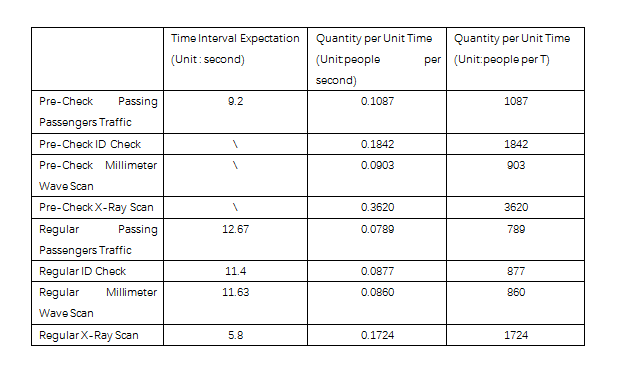
\includegraphics[width=15cm]{p1.png}
\section{Establishing The Model}

\setlength{\parindent}{2em}
The first problem we need solve is to discover the bottlenecks of airport security system. To know where the bottlenecks lie, the model is firstly needed to calculate the upper limit of airport security efficiency. Airport security efficiency is reflected in the time interval between the two neighboring people having passed checkpoints. The smaller the mathematical expectations of the time interval is, the higher the efficiency is, and it is equal that, the larger the passing passenger quantity is, the higher the efficiency is. So we can map the passing number per unit time as the network traffic to the map and obviously edges of the net is steps of security check system. In this model, each step of security check is one-way, which is in line with the conditions of Network-Flows.


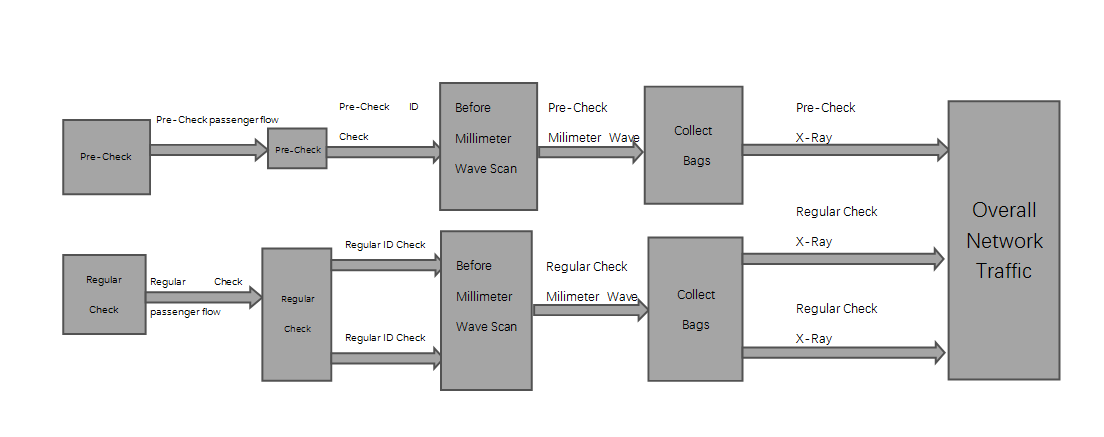
\includegraphics[width=15cm]{m1.png}
Appendix $:$ We just present three channels and according to the rules, only one channel is for Pre-Check in these three channels.

\section{Testing}

\setlength{\parindent}{2em}
Our approach to discover the bottleneck is to modify the capacity of some of the edges in the network and observe the effect on the maximum network traffic. The feasible operation is to assume that the efficiency of a certain channel is increased and observe the effect on the maximum network traffic. For example, if we increase the efficiency of a certain channel and the efficiency is greatly enhanced, we can conclude that there is a certain relationship between this channel and the maximum network traffic.
In order to make a more apparent difference in the efficiency of the different channels, we assume that the inflow of the two types of passengers is doubled.

(1) Test without any changes:

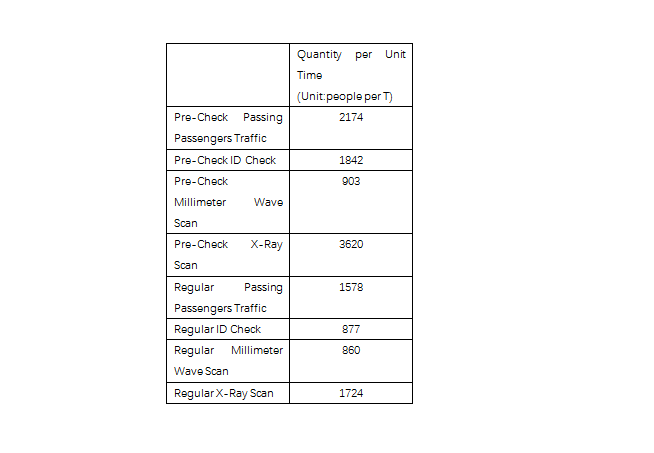
\includegraphics[width=15cm]{p2.png}
     The current maximum network traffic is : 1763


(2) Only increase Pre-Check channel efficiency by 200 people/T and others remain unchanged
The current maximum network traffic is : 1963

(3)Only increase regular check channel efficiency by 200 people/T and others remain unchanged
The current maximum network traffic is : 1963

(4)Only increase Pre-Check channel efficiency by 400 people/T and others remain unchanged
The current maximum network traffic is : 2163

(5)Only increase regular check channel efficiency by 400 people/T and others remain unchanged
The current maximum network traffic is : 2163

(6)Only increase Pre-Check channel efficiency by 600 people/T and others remain unchanged
The current maximum network traffic is : 2363

(7)Only increase regular check channel efficiency by 600 people/T and others remain unchanged
The current maximum network traffic is : 2363

(8)Only increase Pre-Check channel efficiency by 800 people/T and others remain unchanged
The current maximum network traffic is : 2563

(9)Only increase regular check channel efficiency by 800 people/T and others remain unchanged
The current maximum network traffic is : 2481

(10)Only increase Pre-Check channel efficiency by 1000 people/T and others remain unchanged
The current maximum network traffic is : 2763

(11)Only increase regular check channel efficiency by 1000 people/T and others remain unchanged
The current maximum network traffic is : 2481
\section{Result Analysis}

\setlength{\parindent}{2em}
As mentioned above, we find that in the former tests, the influence on the maximum network traffic is the same. While, after we enhance one channel's efficiency by 800 people per T, it is indicated that the Pre-Check channel with increased efficiency gains significantly higher than the benefits of the same increase on regular check channel.
So, we just can imagine that, when we want to enhance overall efficiency through increasing one of the channels and the growth of increase reach a certain degree, continue increasing won't bring the maximum network traffic's growth, but for Pre-Check channel, the growth of overall  maximum network traffic. From the point of practical security check system, it isn't difficult to understand the cause of the test result is that too many people lining up in the Pre-Check channel. Therefore, it is concluded that it is the low efficiency of Pre-Check channel where the bottlenecks lie.
\section{Our Programs}

\setlength{\parindent}{2em}
As introduced above, we find the bottlenecks and we propose our two programs.

(1) make Pre-Check passengers line up in regular check channels when there are too many Pre-Check passengers.


Obviously in fact regular check channels also have the same conflict that too many passengers lining up which causes low efficiency but it is just not so prominent and serious. Without compromising the primary security, it is quite difficult to improve Pre-Check channel efficiency or the upgraded cost is practically high even the effect is not obvious, such as, improving equipment and increasing officers, etc. Thus, it is occurred to us that we can make Pre-Check passengers line up in regular check channels when there are too many Pre-Check passengers. So that it can alleviate the problem to some extent with acceptable cost and high feasibility. We give the corresponding model as followed$:$

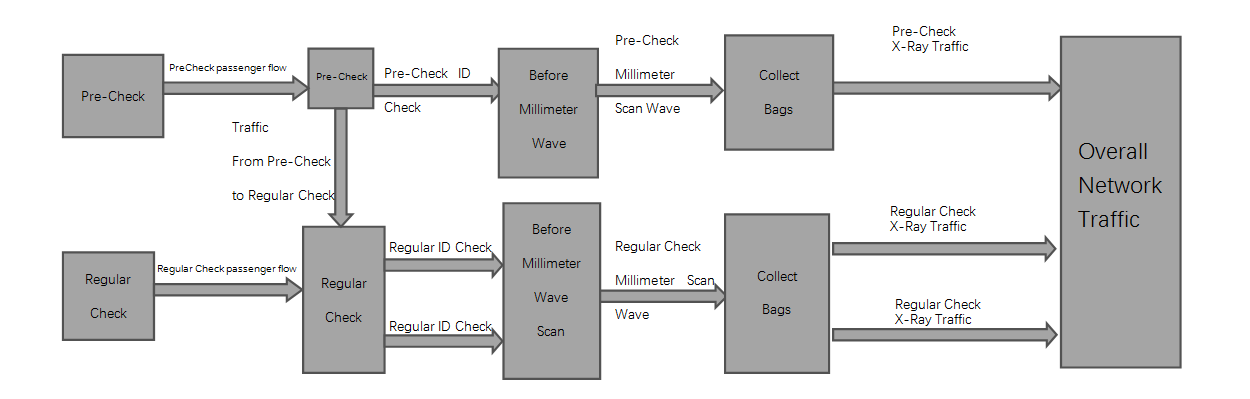
\includegraphics[width=14cm]{m2.png}



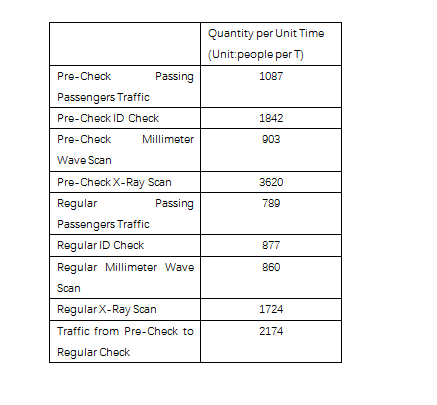
\includegraphics[width=11cm]{p3.png}
The test using Network-Flows$:$
We use the origin given data to calculate the passing passenger traffic of the two types. The rest data remain the same with the origin data.
And the result:
       Before our program:  the maximum network traffic is 1692 people per unit time(T)
       After our program:  the maximum network traffic is 1793 people per unit time(T)
It is concluded that though this program is simple, it indeed enhance the overall security system efficiency and ensure the security of checkpoints.


(2)enable the disabled channel next to the Pre-Check channel
Taking this action is equal to directly increase passing passengers’ quantity to improve the overall efficiency of the airport security system. In this case, we have two ways to achieve it.
One is to add a Pre-Check channel for each three regular check channels which we called Program A and the other is to add a regular check channel. We test the two ways separately to demonstrate which one is the better.
For the purpose of making comparison between two ways more prominent, we still make passing passengers’ traffic of the two types doubled.
We already know the maximum traffic is 1763 people per T through calculations above.
Testing:
 A: add a Pre-Check channel for each three regular check channels

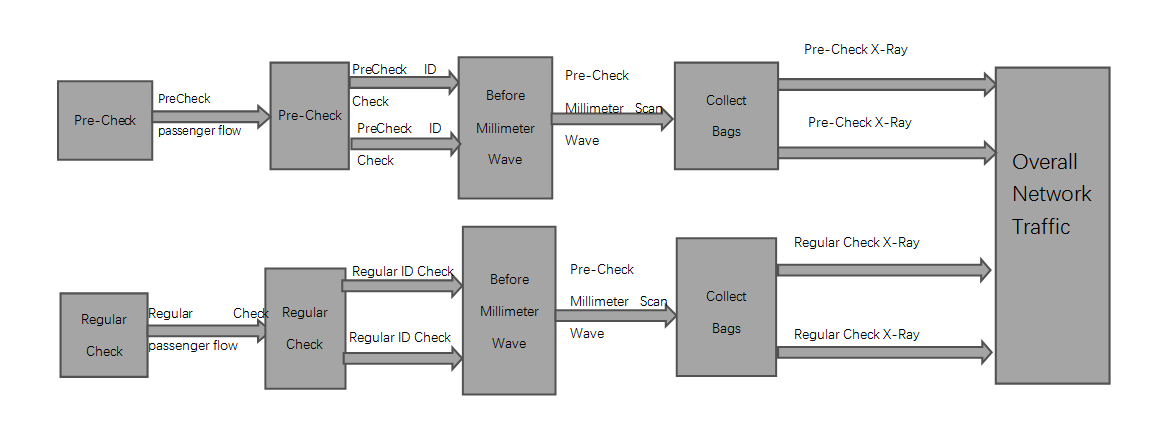
\includegraphics[width=14cm]{m3.png}

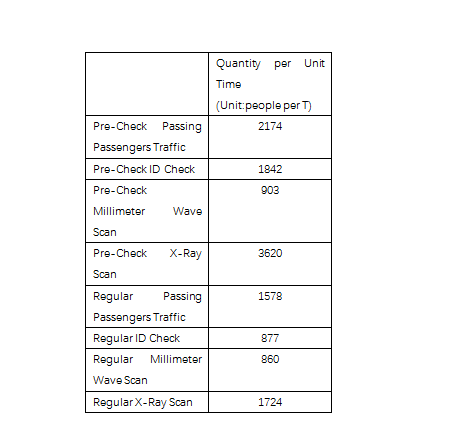
\includegraphics[width=15cm]{p4.png}

We get the result that the maximum network traffic is refreshed to be 2666 people per T.
B: add a regular check channel

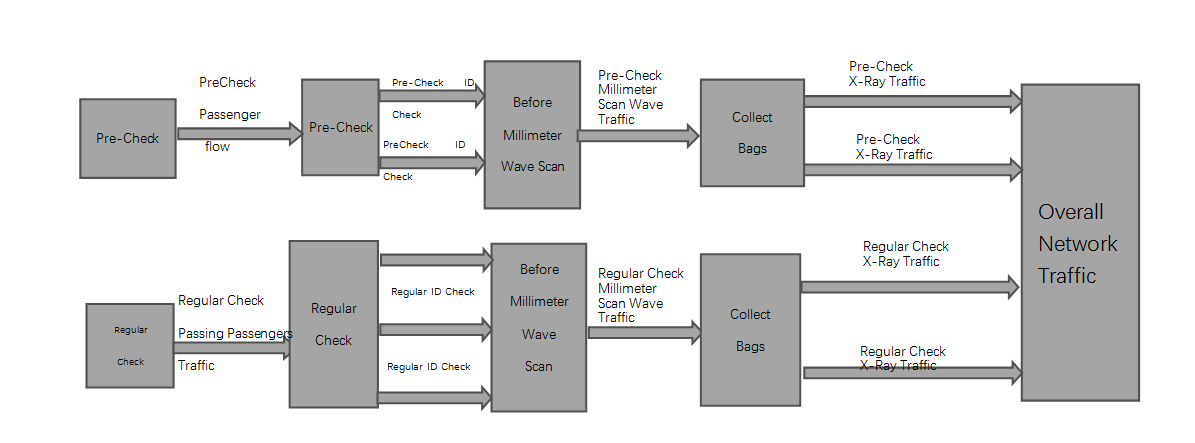
\includegraphics[width=15cm]{m4.png}

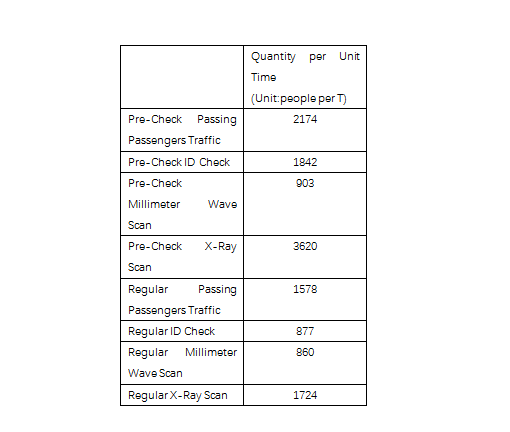
\includegraphics[width=15cm]{p5.png}
We get the result that the maximum network traffic is refreshed to be 2666 people per T.

Obviously, we can conclude that the Program A is better .And in the mean time, this conclusion also conforms the rules. Because the crowding degree of Pre-Check channel is higher than that in regular check channels, it is more necessary for the airport to add Pre-Check channels to alleviate tricky problem.
\section{Evaluate}


\subsection{Merits}

\setlength{\parindent}{2em}
As we all know, Americans emphasize privacy and personal space, so Pre-Check passengers may not be willing to give up the Pre-Check rights to line up in regular check channels. While, Chinese people are more concerned about personal efficiency and Swiss is concerned about collective efficiency so that they can choose the first program. The Pre-Check passengers will choose to give up Pre-Check rights to save their time so that the overall efficiency is enhanced. Besides, cost conditions permitting, for Americans, we can take the second program, adding a Pre-Check channel, which ensure Americans' privacy and can't be more suitable.
What's more, it's easy to visually see the specific processes of an airport security system and directly obtain a certain data representing airport security system efficiency after appropriate treatment on the given data of each security check step.
As long as the case process is unchanged, we can get a result for each time interval conveniently.
\subsection{Drawbacks}

\setlength{\parindent}{2em}
Although our model indeed solve the problem in a certain degree, we have our own disadvantage and not perfectly. For instance, one establishment of our model is just for an airport security system process. If you want to change some checking process, we must establish a new model to apply new system, and for establishing the model, we have prerequisites sometimes, for example, passing passengers traffic is a stable and independent value and we need change this parameter to change efficiency. However, practical situations are not so ideal.
Because different process have influences on each other and the influence usually is not sure. So if we want to modify our model to make it more practical and feasible, we need analyze the influence with each process and the relation between different processes and quantify them into a mathematical relation equation.

\section{References}





\begin{thebibliography}{30}
\bibitem{book}OPTIMIZING PROCESS OF CHECK-IN AND SECURITY
CHECK AT AIRPORT TERMINALS, Jaromir Siroky, Pavlina Hlavsova, December 2014.
\end{thebibliography}

\end{document}


